%% ****** Start of file apstemplate.tex ****** %
%%
%%
%%   This file is part of the APS files in the REVTeX 4.2 distribution.
%%   Version 4.2a of REVTeX, January, 2015
%%
%%
%%   Copyright (c) 2015 The American Physical Society.
%%
%%   See the REVTeX 4 README file for restrictions and more information.
%%
%
% This is a template for producing manuscripts for use with REVTEX 4.2
% Copy this file to another name and then work on that file.
% That way, you always have this original template file to use.
%
% Group addresses by affiliation; use superscriptaddress for long
% author lists, or if there are many overlapping affiliations.
% For Phys. Rev. appearance, change preprint to twocolumn.
% Choose pra, prb, prc, prd, pre, prl, prstab, prstper, or rmp for journal
%  Add 'draft' option to mark overfull boxes with black boxes
%  Add 'showkeys' option to make keywords appear
%\documentclass[aps,prl,preprint,groupedaddress]{revtex4-2}
\documentclass[aps,prl,twocolumn,groupedaddress]{revtex4-2}
%\documentclass[aps,prl,preprint,superscriptaddress]{revtex4-2}
%\documentclass[aps,prl,reprint,groupedaddress]{revtex4-2}

% You should use BibTeX and apsrev.bst for references
% Choosing a journal automatically selects the correct APS
% BibTeX style file (bst file), so only uncomment the line
% below if necessary.
%\bibliographystyle{apsrev4-2}

\usepackage{graphicx}
\usepackage{epstopdf}
%\usepackage{amsmath}% http://ctan.org/pkg/amsmath
%\usepackage{amsthm}
%\usepackage{amsfonts}
%\usepackage{subfigure}
%\usepackage{hhline}
%\usepackage[miktex]{gnuplottex}
%\usepackage{xcolor}
\usepackage{amssymb}
\usepackage{amsmath}
\usepackage{color}
\usepackage[hidelinks]{hyperref}
%\usepackage[percent]{overpic}
\usepackage{tikz}
\usetikzlibrary{arrows.meta,positioning,calc,fit}
\usepackage{mathrsfs}
\usepackage{wasysym}
\usepackage{tikz-cd}
%\usepackage{stix} %\fisheye
\usepackage{stackengine,scalerel}
\usepackage{multirow}

% so sections, subsections, etc. become numerated.
\setcounter{secnumdepth}{3}

% Parámetros de flotantes: los valores por defecto de LaTeX son muy
% restrictivos y, con siete flotantes (varios a doble columna), hacían que
% las figuras se acumularan y aparecieran varias páginas después del texto
% que las cita. Para revertir, basta con borrar este bloque.
\renewcommand{\topfraction}{0.9}        % máx. de página ocupable por flotantes arriba
\renewcommand{\bottomfraction}{0.7}
\renewcommand{\textfraction}{0.07}      % mín. de texto exigido por página
\renewcommand{\floatpagefraction}{0.75}
\renewcommand{\dbltopfraction}{0.9}     % ídem, para flotantes a doble columna
\renewcommand{\dblfloatpagefraction}{0.75}
\setcounter{topnumber}{3}
\setcounter{dbltopnumber}{3}
\setcounter{totalnumber}{4}

% Comandos proprios
\DeclareMathOperator*{\argmax}{arg\,max}
\DeclareMathOperator*{\argmin}{arg\,min}
\newcommand{\avrg}[1]{\left\langle #1 \right\rangle}
\newcommand{\nelta}{\bar{\delta}}
\newcommand{\bra}[1]{\left\langle #1\right|}
\newcommand{\ket}[1]{\left| #1 \right\rangle}
\newcommand{\sbra}[1]{\langle #1|}
\newcommand{\sket}[1]{| #1 \rangle}
\newcommand{\bek}[3]{\left\langle #1 \right| #2 \left| #3 \right\rangle}
\newcommand{\sbek}[3]{\langle #1 | #2 | #3 \rangle}
\newcommand{\braket}[2]{\left\langle #1 \middle| #2 \right\rangle}
\newcommand{\ketbra}[2]{\left| #1 \middle\rangle \middle\langle #2  \right|}
\newcommand{\sbraket}[2]{\langle #1 | #2 \rangle}
\newcommand{\sketbra}[2]{| #1 \rangle  \langle #2 |}
\newcommand{\norm}[1]{\left\lVert#1\right\rVert}
\newcommand{\snorm}[1]{\lVert#1\rVert}
\newcommand{\bvec}[1]{\boldsymbol{\mathsf{#1}}}
\newcommand{\bcov}[1]{\boldsymbol{#1}}
\newcommand{\bdua}[1]{\boldsymbol{\check{#1}}}
%\newcommand{\bdov}[1]{\boldsymbol{\breve{#1}}}
\newcommand{\bdov}[1]{\breve{#1}}
%\newcommand{\bten}[1]{\boldsymbol{\mathfrak{#1}}}
\newcommand{\bten}[1]{\boldsymbol{\mathfrak{#1}}}
\newcommand{\forany}{\tilde{\forall}}
\newcommand{\qed}{$\overset{\circ}{.}\;$}

\newcommand\bigeye{\ensurestackMath{\stackinset{c}{}{c}{-.3pt}%
  {\bullet}{\scriptstyle\bigcirc}}}
\newcommand\eye{\scalerel*{\bigeye}{x}}
%\newcommand*{\fisheye}{%
%    \mathbin{%
%        \ooalign{$\circledcirc$\cr\hidewidth$\bullet$\hidewidth}%
%    }%
%}
\renewcommand{\appendixname}{Apéndice}

\begin{document}

% Use the \preprint command to place your local institutional report
% number in the upper righthand corner of the title page in preprint mode.
% Multiple \preprint commands are allowed.
% Use the 'preprintnumbers' class option to override journal defaults
% to display numbers if necessary
%\preprint{}

%Title of paper
\title{
Restauración de imágenes con MAXIM y Mixture of Experts
}

% repeat the \author .. \affiliation  etc. as needed
% \email, \thanks, \homepage, \altaffiliation all apply to the current
% author. Explanatory text should go in the []'s, actual e-mail
% address or url should go in the {}'s for \email and \homepage.
% Please use the appropriate macro foreach each type of information

% \affiliation command applies to all authors since the last
% \affiliation command. The \affiliation command should follow the
% other information
% \affiliation can be followed by \email, \homepage, \thanks as well.
\author{Matías Ariel Murat}
% \email[]{matias.murat@mi.unc.edu.ar}
\affiliation{Facultad de Matem\'atica, Astronom\'ia, F\'isica y Computaci\'on, Universidad Nacional de C\'ordoba, Ciudad Universitaria, 5000 C\'ordoba, Argentina}

%Collaboration name if desired (requires use of superscriptaddress
%option in \documentclass). \noaffiliation is required (may also be
%used with the \author command).
%\collaboration can be followed by \email, \homepage, \thanks as well.
%\collaboration{Juan Perez}
%\noaffiliation

% \date{\today}

\begin{abstract}
Este trabajo aborda la restauración de imágenes mediante una variante de MAXIM (Multi-Axis MLP) con un esquema de Mixture of Experts (MoE), que combina un backbone compartido con un ruteador que pondera dinámicamente un conjunto de cabezas expertas de reconstrucción, buscando especialización sin duplicar el costo de las etapas profundas. Sobre un conjunto unificado de cinco tareas, las versiones multi-tarea de MAXIM sin MoE alcanzan entre $24{,}8$ y $25{,}5$~dB de PSNR de validación (una versión mono-tarea de referencia, especializada únicamente en realce, llega a $24{,}0$~dB sobre esa única tarea), mientras que la variante MAXIM+MoE converge a $23{,}4$~dB: entrena de forma estable y produce reconstrucciones competentes, pero no supera a una versión sin MoE de idéntica escala e inicialización ($24{,}8$~dB), y su ruteador converge a un régimen prácticamente uniforme sin que emerja especialización entre expertos. Analizamos por qué la mezcla no aporta ---una regularización que premia el ruteo uniforme y un ruteo denso sobre cabezas expertas de capacidad mínima que quedan casi idénticas--- y derivamos líneas concretas de mejora. El resultado, negativo pero informativo, delimita las condiciones bajo las cuales la especialización tardía por expertos podría aportar valor en restauración de imágenes.
\end{abstract}

% insert suggested keywords - APS authors don't need to do this
%\keywords{}

%\maketitle must follow title, authors, abstract, and keywords
\maketitle

\section{Introducción}

La restauración de imágenes es un problema central en visión por computadora de bajo nivel. En la práctica, las imágenes pueden verse degradadas por ruido, desenfoque, baja iluminación u otros factores, y cada tipo de degradación suele requerir estrategias de reconstrucción con sesgos diferentes. En este contexto, un único camino de procesamiento puede resultar limitado cuando se busca robustez frente a distribuciones heterogéneas.

MAXIM~\cite{tu2022maxim} constituye una alternativa relevante dentro de las arquitecturas recientes para restauración de imágenes, ya que combina operaciones locales y globales con un diseño completamente convolucional. Sin embargo, en su formulación estándar, el modelo mantiene un flujo de cómputo uniforme para todas las entradas. Esta característica simplifica el diseño, pero reduce su capacidad de especialización frente a escenarios diversos.

Para abordar ese punto, en este trabajo se propone integrar el paradigma Mixture of Experts (MoE)~\cite{jacobs1991mixtures,shazeer2017moe} sobre MAXIM. La idea principal es mantener un backbone compartido para preservar eficiencia y, sobre la representación latente obtenida, aplicar un mecanismo de ruteo que pondere para cada entrada un conjunto de expertos de salida especializados.

Los objetivos de este trabajo son:
\begin{itemize}
    \item Diseñar una variante MAXIM+MoE compatible con restricciones de memoria y entrenamiento.
    \item Definir un protocolo experimental claro para evaluar calidad de reconstrucción y costo computacional.
    \item Analizar, mediante resultados cuantitativos y el diagnóstico del ruteador, en qué medida la especialización por expertos aporta frente a una versión sin MoE.
\end{itemize}

La organización del documento es la siguiente. En la Sección~II se presentan los fundamentos teóricos de MAXIM y de MoE. En la Sección~III se detalla la metodología implementada: arquitectura, datos, protocolo de entrenamiento y métricas. La Sección~IV reporta los resultados cuantitativos de las cuatro configuraciones entrenadas y el análisis del ruteador. Las Secciones~V y~VI discuten los hallazgos y presentan las conclusiones, y la Sección~VII delinea el trabajo futuro.

\section{Teoría}

\subsection{MAXIM como arquitectura base}

MAXIM (Multi-Axis MLP) es una arquitectura orientada a tareas de restauración de imágenes. Su diseño general sigue una estructura tipo U, donde las conexiones skip permiten combinar información de bajo y alto nivel. A diferencia de enfoques puramente convolucionales, MAXIM incorpora bloques MLP con mecanismos de compuerta que capturan interacciones de largo alcance.

La arquitectura se apoya principalmente en dos módulos. El primero es el bloque \textit{multi-axis gated MLP}, que permite modelar interacciones locales y globales entre elementos visuales a través de compuertas aplicadas sobre distintos ejes de la representación. El segundo es el bloque de compuertas cruzadas, propuesto como una alternativa basada en MLP a mecanismos de atención cruzada. En conjunto, estos módulos permiten incorporar contexto global sin abandonar una estructura eficiente para el procesamiento de imágenes.

Una propiedad importante de esta arquitectura es que mantiene una naturaleza completamente convolucional en el flujo de entrada y salida. Esto permite procesar imágenes de tamaño variable sin rediseñar el modelo para cada resolución. Además, MAXIM expresa campos receptivos globales sobre imágenes arbitrariamente grandes con un costo que escala linealmente con el tamaño de la entrada, evitando el crecimiento cuadrático típico de mecanismos de atención global directa.

El diseño también integra varias ideas frecuentes en visión de bajo nivel, como aprendizaje residual, conexiones densas, estructuras jerárquicas, procesamiento en múltiples etapas y mecanismos de atención o compuerta. Su combinación de bloques locales convolucionales y bloques globales basados en MLP logran un balance útil entre preservación de detalle fino y uso de contexto amplio, logrando buen desempeño sin depender necesariamente de preentrenamiento a gran escala.

MAXIM está implementado usando Flax, una librería Python de redes neuronales construida sobre JAX, una librería de computación numérica de alto rendimiento. Flax/JAX permiten usar diferenciación automática o algorítmica, más eficiente que los métodos clásicos de diferenciación numérica o simbólica. Otra ventaja de JAX es que permite la compilación JIT (\textit{just-in-time}), una técnica que combina interpretación y compilación. Consiste en compilar y optimizar dinámicamente los métodos más usados durante la ejecución, combinando ventajas como la velocidad del código compilado y la flexibilidad del interpretado.


\subsection{Paradigma Mixture of Experts}

Mixture of Experts (MoE) es un paradigma de modelado en el cual varios submódulos especialistas (expertos) colaboran bajo un mecanismo de ruteo. El ruteador recibe una representación de la entrada y estima qué experto, o conjunto reducido de expertos, es más apropiado para producir la salida.

La motivación principal de MoE es aumentar la capacidad de representación sin activar todos los parámetros para cada muestra. De este modo, el sistema puede adaptarse mejor a datos heterogéneos, manteniendo controlado el costo computacional efectivo por inferencia.

El ruteo admite distintas variantes. En el ruteo \textit{disperso} (\textit{sparse}) se selecciona únicamente el experto de mayor peso (top-1) o los dos de mayor peso (top-2), de modo que solo una fracción de los expertos se evalúa por muestra~\cite{shazeer2017moe,fedus2022switch}. En el ruteo \textit{denso} o \textit{suave}, en cambio, todos los expertos se evalúan y la salida es una combinación convexa de sus predicciones, ponderada por una distribución \textit{softmax} sobre los pesos de compuerta. La variante densa es más simple y diferenciable de extremo a extremo, pero no reduce el cómputo y, como se verá, es más propensa a soluciones de ruteo poco discriminativas.

En el contexto de restauración de imágenes, esta idea resulta relevante porque un único modelo puede recibir entradas afectadas por degradaciones distintas, como ruido, desenfoque, baja iluminación o compresiones con diferentes características. Un camino de cómputo compartido debe representar todos esos casos con los mismos parámetros activos, mientras que un esquema MoE permite dividir implícitamente el problema en subconjuntos y asignar expertos a patrones de degradación o regiones del espacio de datos.

\subsection{Integración MAXIM+MoE propuesta}

En este trabajo no se replica el backbone completo de MAXIM para cada experto. En cambio, se usa un único extractor compartido de características profundas y se aplica la especialización en la etapa de reconstrucción final. En términos conceptuales, dado un mapa de características $f_\theta(x)$, la salida se modela como:
\begin{equation}
\hat{y} = \sum_{k=1}^{K} p_k(x)\, E_k(f_\theta(x)),
\end{equation}
donde $E_k$ representa al experto $k$ y $p_k(x)$ es el peso asignado por el ruteador para la entrada $x$.

Esta formulación habilita un gradiente de especialización entre expertos sin multiplicar el costo de las capas profundas de MAXIM. La decisión responde a una restricción práctica del proyecto: la replicación completa de bloques globales incrementa fuertemente el consumo de memoria y dificulta el entrenamiento estable con recursos limitados.

En este esquema, los expertos no procesan directamente la imagen degradada ni intervienen en las primeras etapas de extracción de características. Cada experto funciona como una cabeza de salida especializada que opera sobre la representación latente producida por MAXIM. Por lo tanto, el ruteador puede interpretarse como un selector de hipótesis de reconstrucción: a partir de las características globales de la entrada, pondera las salidas expertas que mejor se ajustan al caso observado.

Este enfoque conserva las ventajas centrales de MAXIM, como su carácter completamente convolucional y su capacidad para operar sobre resoluciones arbitrarias, pero introduce especialización con un incremento marginal respecto del costo del backbone. La propuesta puede verse como un compromiso entre capacidad y eficiencia: la especialización ocurre en una etapa tardía, aunque sobre representaciones suficientemente ricas para capturar variaciones complejas en la reconstrucción.

\subsection{Consideraciones de entrenamiento}

La integración de MoE introduce desafíos específicos. El más conocido es el \textit{colapso del ruteador}: el sistema puede converger a usar siempre el mismo experto, o bien al extremo opuesto, repartir la carga de forma idéntica entre todos los expertos sin diferenciarlos. Para mitigar el primer caso es habitual añadir un término de \textit{balance de carga} que penaliza distribuciones de uso muy desiguales~\cite{shazeer2017moe,fedus2022switch}, y un término de \textit{entropía} que regula cuán concentrada o dispersa es la distribución de compuerta. Estos términos deben calibrarse con cuidado: una regularización demasiado fuerte hacia el balance empuja precisamente hacia el segundo modo de colapso, en el que el ruteo se vuelve uniforme y deja de aportar especialización.

Por ese motivo, el protocolo metodológico contempla estos criterios de balance y un monitoreo explícito de la utilización por experto. Con este marco teórico, la siguiente sección describe el diseño experimental adoptado para implementar y evaluar la variante MAXIM+MoE.

\section{Metodología}

\subsection{Diseño del modelo}

La arquitectura implementada (Fig.~\ref{fig:arch}) se compone de tres partes:
\begin{itemize}
    \item un backbone MAXIM compartido, encargado de extraer representaciones latentes a partir de la imagen degradada;
    \item un módulo de ruteo, que a partir de la imagen de entrada estima una distribución de pesos sobre los expertos;
    \item un conjunto de $K$ cabezas expertas de salida, cada una encargada de la proyección desde la representación latente hacia la imagen restaurada.
\end{itemize}

\begin{figure*}[t]
\centering
% =====================================================================
%  fig_arch.tex  --  Vista general de la arquitectura MAXIM+MoE
%
%  Uso en main.tex (dentro de un figure*):   % =====================================================================
%  fig_arch.tex  --  Vista general de la arquitectura MAXIM+MoE
%
%  Uso en main.tex (dentro de un figure*):   % =====================================================================
%  fig_arch.tex  --  Vista general de la arquitectura MAXIM+MoE
%
%  Uso en main.tex (dentro de un figure*):   \input{figs/fig_arch}
%
%  REQUIERE en el preámbulo:
%     \usepackage{tikz}
%     \usetikzlibrary{arrows.meta,positioning,calc,fit}
%
%  Vista previa aislada: compilar figs/fig_arch_standalone.tex
% =====================================================================

% --- miniatura de imagen (placeholder dibujado) ----------------------
% Para usar imágenes reales, reemplazar el cuerpo por:
%   \node[inner sep=0pt] (#1) at #2 {\includegraphics[width=10mm]{archivo}};
\providecommand{\imgnode}[3]{%
  \node[draw=black!55,line width=.4pt,minimum size=10mm,inner sep=0pt,fill=#3] (#1) at #2 {};
  \begin{scope}
    \clip ([xshift=.5pt,yshift=.5pt]#1.south west) rectangle ([xshift=-.5pt,yshift=-.5pt]#1.north east);
    \fill[green!35!black!55] (#1.south west) rectangle ([yshift=3.2mm]#1.south east);
    \fill[yellow!75!orange]  ([shift={(-2.7mm,-2.7mm)}]#1.north east) circle (1.1mm);
    \draw[white!80!black,line width=.4pt]
      ([yshift=3.2mm]#1.south west) -- ([shift={(2.1mm,5.6mm)}]#1.south west)
      -- ([shift={(4.6mm,3.2mm)}]#1.south west);
  \end{scope}
}

% --- estilos (definidos al nivel superior, con prefijo m-) -----------
% Se redefinen sin problema si este archivo se incluye junto a fig_moehead.tex.
\tikzset{mblk/.style={draw,rounded corners=1.5pt,minimum height=5.5mm,
                      minimum width=12mm,align=center,inner sep=1.2pt,line width=.4pt}}
\tikzset{menc/.style={mblk,fill=blue!10,draw=blue!60!black}}
\tikzset{mdec/.style={mblk,fill=green!14,draw=green!45!black}}
\tikzset{mbot/.style={mblk,fill=orange!20,draw=orange!70!black}}
\tikzset{mcgb/.style={mblk,fill=red!12,draw=red!60!black,minimum width=9mm}}
\tikzset{mrt/.style={mblk,fill=violet!12,draw=violet!65!black,minimum width=20mm}}
\tikzset{mex/.style={mblk,fill=yellow!28,draw=olive!80!black,minimum width=15mm}}
\tikzset{mgrp/.style={draw=black!45,dashed,rounded corners=3pt,line width=.4pt}}
\tikzset{mop/.style={draw,circle,minimum size=3.6mm,inner sep=0pt,line width=.4pt}}
\tikzset{mar/.style={->,line width=.45pt}}
\tikzset{mgate/.style={->,line width=.45pt,densely dashed,draw=violet!70!black}}
\tikzset{mcap/.style={font=\scriptsize,align=center}}

\begin{tikzpicture}[font=\scriptsize,>={Stealth[length=4pt,width=3pt]}]

% --- entrada ---------------------------------------------------------
\imgnode{xin}{(0,0)}{blue!14!gray!35}
\node[mcap,below=1.2mm of xin] {$x$\\ \itshape degradada};

% --- backbone MAXIM: glifo tipo U-Net --------------------------------
\node[menc] (e1) at (2.35, 1.15) {Encoder};
\node[menc] (e2) at (2.35, 0.35) {Encoder};
\node[menc] (e3) at (2.35,-0.45) {Encoder};
\node[mcgb] (c1) at (3.95, 1.15) {CGB};
\node[mcgb] (c2) at (3.95, 0.35) {CGB};
\node[mcgb] (c3) at (3.95,-0.45) {CGB};
\node[mdec] (d1) at (5.55, 1.15) {Decoder};
\node[mdec] (d2) at (5.55, 0.35) {Decoder};
\node[mdec] (d3) at (5.55,-0.45) {Decoder};
\node[mbot] (bn) at (3.95,-1.25) {Bottleneck};

\draw[mar] (e1) -- node[right,pos=.42,font=\tiny,inner sep=1pt] {$\downarrow$2} (e2);
\draw[mar] (e2) -- node[right,pos=.42,font=\tiny,inner sep=1pt] {$\downarrow$2} (e3);
\draw[mar] (e3.south) |- (bn.west);
\draw[mar] (bn.east) -| (d3.south);
\draw[mar] (d3) -- node[right,pos=.42,font=\tiny,inner sep=1pt] {$\uparrow$2} (d2);
\draw[mar] (d2) -- node[right,pos=.42,font=\tiny,inner sep=1pt] {$\uparrow$2} (d1);

% skips a través de los bloques de compuertas cruzadas
\draw[mar] (e1) -- (c1);  \draw[mar] (c1) -- (d1);
\draw[mar] (e2) -- (c2);  \draw[mar] (c2) -- (d2);
\draw[mar] (e3) -- (c3);  \draw[mar] (c3) -- (d3);

% features globales propagadas hacia arriba
\draw[mar,draw=black!45] (bn.north) -- (c3.south);
\draw[mar,draw=black!45] (c3) -- (c2);
\draw[mar,draw=black!45] (c2) -- (c1);

\node[mgrp,fit=(e1)(d1)(bn),inner sep=3.2mm] (bbox) {};
\node[mcap,above=0.8mm of bbox.north]
  {\textbf{Backbone MAXIM} ($\theta$), variante S-2, $\times 2$ etapas};
\draw[mar] (xin.east) -- (bbox.west);

% --- mapa de características -----------------------------------------
\draw[fill=teal!8 ,draw=teal!60!black,line width=.4pt] (7.30,-0.55) rectangle (8.00,0.55);
\draw[fill=teal!16,draw=teal!60!black,line width=.4pt] (7.45,-0.40) rectangle (8.15,0.70);
\draw[fill=teal!26,draw=teal!60!black,line width=.4pt] (7.60,-0.25) rectangle (8.30,0.85);
\coordinate (fmapW) at (7.30,0.15);
\coordinate (fmapE) at (8.30,0.15);
\node[mcap] at (7.80,-1.10) {$f_\theta(x)$\\ $H\!\times\!W\!\times\!C$};
\draw[mar] (bbox.east) -- (fmapW);

% --- cabezal MoE (resumido; el detalle está en la otra figura) --------
\node[mblk,minimum width=23mm,minimum height=18mm,fill=yellow!14,draw=olive!80!black]
  (moebox) at (10.2,0.15) {\textbf{MoE Header}\\ $K=5$ expertos $+$ router};
\draw[mar] (fmapE) -- (moebox.west);

% --- ruteador ---------------------------------------------------------
\node[mrt,minimum width=34mm,minimum height=10mm] (rt) at (5.0,-2.60)
  {Router $g_\phi$ \\ conv.\ separables $+$ MLP $\rightarrow$ softmax};
\draw[mar] (xin.west) -- ++(-0.45,0) |- (rt.west);
\draw[mgate] (rt.east) -| node[pos=.22,above,font=\tiny,inner sep=1.5pt] {$p(x)\in\Delta^{K-1}$} (moebox.south);

% --- salida -----------------------------------------------------------
\imgnode{yout}{(12.5,0.15)}{blue!25!white}
\node[mcap,below=1.2mm of yout] {$\hat{y}$\\ \itshape restaurada};
\draw[mar] (moebox.east) -- (yout.west);

% --- conexión residual global -----------------------------------------
\draw[mar,draw=black!55] (xin.north) -- (0,2.80) -- (12.5,2.80) -- (yout.north);
\node[mcap,above=0.3mm] at (6.3,2.80)
  {conexión residual:\; $\hat{y}=x+\sum_{k=1}^{K} p_k(x)\,E_k\!\big(f_\theta(x)\big)$};

\end{tikzpicture}

%
%  REQUIERE en el preámbulo:
%     \usepackage{tikz}
%     \usetikzlibrary{arrows.meta,positioning,calc,fit}
%
%  Vista previa aislada: compilar figs/fig_arch_standalone.tex
% =====================================================================

% --- miniatura de imagen (placeholder dibujado) ----------------------
% Para usar imágenes reales, reemplazar el cuerpo por:
%   \node[inner sep=0pt] (#1) at #2 {\includegraphics[width=10mm]{archivo}};
\providecommand{\imgnode}[3]{%
  \node[draw=black!55,line width=.4pt,minimum size=10mm,inner sep=0pt,fill=#3] (#1) at #2 {};
  \begin{scope}
    \clip ([xshift=.5pt,yshift=.5pt]#1.south west) rectangle ([xshift=-.5pt,yshift=-.5pt]#1.north east);
    \fill[green!35!black!55] (#1.south west) rectangle ([yshift=3.2mm]#1.south east);
    \fill[yellow!75!orange]  ([shift={(-2.7mm,-2.7mm)}]#1.north east) circle (1.1mm);
    \draw[white!80!black,line width=.4pt]
      ([yshift=3.2mm]#1.south west) -- ([shift={(2.1mm,5.6mm)}]#1.south west)
      -- ([shift={(4.6mm,3.2mm)}]#1.south west);
  \end{scope}
}

% --- estilos (definidos al nivel superior, con prefijo m-) -----------
% Se redefinen sin problema si este archivo se incluye junto a fig_moehead.tex.
\tikzset{mblk/.style={draw,rounded corners=1.5pt,minimum height=5.5mm,
                      minimum width=12mm,align=center,inner sep=1.2pt,line width=.4pt}}
\tikzset{menc/.style={mblk,fill=blue!10,draw=blue!60!black}}
\tikzset{mdec/.style={mblk,fill=green!14,draw=green!45!black}}
\tikzset{mbot/.style={mblk,fill=orange!20,draw=orange!70!black}}
\tikzset{mcgb/.style={mblk,fill=red!12,draw=red!60!black,minimum width=9mm}}
\tikzset{mrt/.style={mblk,fill=violet!12,draw=violet!65!black,minimum width=20mm}}
\tikzset{mex/.style={mblk,fill=yellow!28,draw=olive!80!black,minimum width=15mm}}
\tikzset{mgrp/.style={draw=black!45,dashed,rounded corners=3pt,line width=.4pt}}
\tikzset{mop/.style={draw,circle,minimum size=3.6mm,inner sep=0pt,line width=.4pt}}
\tikzset{mar/.style={->,line width=.45pt}}
\tikzset{mgate/.style={->,line width=.45pt,densely dashed,draw=violet!70!black}}
\tikzset{mcap/.style={font=\scriptsize,align=center}}

\begin{tikzpicture}[font=\scriptsize,>={Stealth[length=4pt,width=3pt]}]

% --- entrada ---------------------------------------------------------
\imgnode{xin}{(0,0)}{blue!14!gray!35}
\node[mcap,below=1.2mm of xin] {$x$\\ \itshape degradada};

% --- backbone MAXIM: glifo tipo U-Net --------------------------------
\node[menc] (e1) at (2.35, 1.15) {Encoder};
\node[menc] (e2) at (2.35, 0.35) {Encoder};
\node[menc] (e3) at (2.35,-0.45) {Encoder};
\node[mcgb] (c1) at (3.95, 1.15) {CGB};
\node[mcgb] (c2) at (3.95, 0.35) {CGB};
\node[mcgb] (c3) at (3.95,-0.45) {CGB};
\node[mdec] (d1) at (5.55, 1.15) {Decoder};
\node[mdec] (d2) at (5.55, 0.35) {Decoder};
\node[mdec] (d3) at (5.55,-0.45) {Decoder};
\node[mbot] (bn) at (3.95,-1.25) {Bottleneck};

\draw[mar] (e1) -- node[right,pos=.42,font=\tiny,inner sep=1pt] {$\downarrow$2} (e2);
\draw[mar] (e2) -- node[right,pos=.42,font=\tiny,inner sep=1pt] {$\downarrow$2} (e3);
\draw[mar] (e3.south) |- (bn.west);
\draw[mar] (bn.east) -| (d3.south);
\draw[mar] (d3) -- node[right,pos=.42,font=\tiny,inner sep=1pt] {$\uparrow$2} (d2);
\draw[mar] (d2) -- node[right,pos=.42,font=\tiny,inner sep=1pt] {$\uparrow$2} (d1);

% skips a través de los bloques de compuertas cruzadas
\draw[mar] (e1) -- (c1);  \draw[mar] (c1) -- (d1);
\draw[mar] (e2) -- (c2);  \draw[mar] (c2) -- (d2);
\draw[mar] (e3) -- (c3);  \draw[mar] (c3) -- (d3);

% features globales propagadas hacia arriba
\draw[mar,draw=black!45] (bn.north) -- (c3.south);
\draw[mar,draw=black!45] (c3) -- (c2);
\draw[mar,draw=black!45] (c2) -- (c1);

\node[mgrp,fit=(e1)(d1)(bn),inner sep=3.2mm] (bbox) {};
\node[mcap,above=0.8mm of bbox.north]
  {\textbf{Backbone MAXIM} ($\theta$), variante S-2, $\times 2$ etapas};
\draw[mar] (xin.east) -- (bbox.west);

% --- mapa de características -----------------------------------------
\draw[fill=teal!8 ,draw=teal!60!black,line width=.4pt] (7.30,-0.55) rectangle (8.00,0.55);
\draw[fill=teal!16,draw=teal!60!black,line width=.4pt] (7.45,-0.40) rectangle (8.15,0.70);
\draw[fill=teal!26,draw=teal!60!black,line width=.4pt] (7.60,-0.25) rectangle (8.30,0.85);
\coordinate (fmapW) at (7.30,0.15);
\coordinate (fmapE) at (8.30,0.15);
\node[mcap] at (7.80,-1.10) {$f_\theta(x)$\\ $H\!\times\!W\!\times\!C$};
\draw[mar] (bbox.east) -- (fmapW);

% --- cabezal MoE (resumido; el detalle está en la otra figura) --------
\node[mblk,minimum width=23mm,minimum height=18mm,fill=yellow!14,draw=olive!80!black]
  (moebox) at (10.2,0.15) {\textbf{MoE Header}\\ $K=5$ expertos $+$ router};
\draw[mar] (fmapE) -- (moebox.west);

% --- ruteador ---------------------------------------------------------
\node[mrt,minimum width=34mm,minimum height=10mm] (rt) at (5.0,-2.60)
  {Router $g_\phi$ \\ conv.\ separables $+$ MLP $\rightarrow$ softmax};
\draw[mar] (xin.west) -- ++(-0.45,0) |- (rt.west);
\draw[mgate] (rt.east) -| node[pos=.22,above,font=\tiny,inner sep=1.5pt] {$p(x)\in\Delta^{K-1}$} (moebox.south);

% --- salida -----------------------------------------------------------
\imgnode{yout}{(12.5,0.15)}{blue!25!white}
\node[mcap,below=1.2mm of yout] {$\hat{y}$\\ \itshape restaurada};
\draw[mar] (moebox.east) -- (yout.west);

% --- conexión residual global -----------------------------------------
\draw[mar,draw=black!55] (xin.north) -- (0,2.80) -- (12.5,2.80) -- (yout.north);
\node[mcap,above=0.3mm] at (6.3,2.80)
  {conexión residual:\; $\hat{y}=x+\sum_{k=1}^{K} p_k(x)\,E_k\!\big(f_\theta(x)\big)$};

\end{tikzpicture}

%
%  REQUIERE en el preámbulo:
%     \usepackage{tikz}
%     \usetikzlibrary{arrows.meta,positioning,calc,fit}
%
%  Vista previa aislada: compilar figs/fig_arch_standalone.tex
% =====================================================================

% --- miniatura de imagen (placeholder dibujado) ----------------------
% Para usar imágenes reales, reemplazar el cuerpo por:
%   \node[inner sep=0pt] (#1) at #2 {\includegraphics[width=10mm]{archivo}};
\providecommand{\imgnode}[3]{%
  \node[draw=black!55,line width=.4pt,minimum size=10mm,inner sep=0pt,fill=#3] (#1) at #2 {};
  \begin{scope}
    \clip ([xshift=.5pt,yshift=.5pt]#1.south west) rectangle ([xshift=-.5pt,yshift=-.5pt]#1.north east);
    \fill[green!35!black!55] (#1.south west) rectangle ([yshift=3.2mm]#1.south east);
    \fill[yellow!75!orange]  ([shift={(-2.7mm,-2.7mm)}]#1.north east) circle (1.1mm);
    \draw[white!80!black,line width=.4pt]
      ([yshift=3.2mm]#1.south west) -- ([shift={(2.1mm,5.6mm)}]#1.south west)
      -- ([shift={(4.6mm,3.2mm)}]#1.south west);
  \end{scope}
}

% --- estilos (definidos al nivel superior, con prefijo m-) -----------
% Se redefinen sin problema si este archivo se incluye junto a fig_moehead.tex.
\tikzset{mblk/.style={draw,rounded corners=1.5pt,minimum height=5.5mm,
                      minimum width=12mm,align=center,inner sep=1.2pt,line width=.4pt}}
\tikzset{menc/.style={mblk,fill=blue!10,draw=blue!60!black}}
\tikzset{mdec/.style={mblk,fill=green!14,draw=green!45!black}}
\tikzset{mbot/.style={mblk,fill=orange!20,draw=orange!70!black}}
\tikzset{mcgb/.style={mblk,fill=red!12,draw=red!60!black,minimum width=9mm}}
\tikzset{mrt/.style={mblk,fill=violet!12,draw=violet!65!black,minimum width=20mm}}
\tikzset{mex/.style={mblk,fill=yellow!28,draw=olive!80!black,minimum width=15mm}}
\tikzset{mgrp/.style={draw=black!45,dashed,rounded corners=3pt,line width=.4pt}}
\tikzset{mop/.style={draw,circle,minimum size=3.6mm,inner sep=0pt,line width=.4pt}}
\tikzset{mar/.style={->,line width=.45pt}}
\tikzset{mgate/.style={->,line width=.45pt,densely dashed,draw=violet!70!black}}
\tikzset{mcap/.style={font=\scriptsize,align=center}}

\begin{tikzpicture}[font=\scriptsize,>={Stealth[length=4pt,width=3pt]}]

% --- entrada ---------------------------------------------------------
\imgnode{xin}{(0,0)}{blue!14!gray!35}
\node[mcap,below=1.2mm of xin] {$x$\\ \itshape degradada};

% --- backbone MAXIM: glifo tipo U-Net --------------------------------
\node[menc] (e1) at (2.35, 1.15) {Encoder};
\node[menc] (e2) at (2.35, 0.35) {Encoder};
\node[menc] (e3) at (2.35,-0.45) {Encoder};
\node[mcgb] (c1) at (3.95, 1.15) {CGB};
\node[mcgb] (c2) at (3.95, 0.35) {CGB};
\node[mcgb] (c3) at (3.95,-0.45) {CGB};
\node[mdec] (d1) at (5.55, 1.15) {Decoder};
\node[mdec] (d2) at (5.55, 0.35) {Decoder};
\node[mdec] (d3) at (5.55,-0.45) {Decoder};
\node[mbot] (bn) at (3.95,-1.25) {Bottleneck};

\draw[mar] (e1) -- node[right,pos=.42,font=\tiny,inner sep=1pt] {$\downarrow$2} (e2);
\draw[mar] (e2) -- node[right,pos=.42,font=\tiny,inner sep=1pt] {$\downarrow$2} (e3);
\draw[mar] (e3.south) |- (bn.west);
\draw[mar] (bn.east) -| (d3.south);
\draw[mar] (d3) -- node[right,pos=.42,font=\tiny,inner sep=1pt] {$\uparrow$2} (d2);
\draw[mar] (d2) -- node[right,pos=.42,font=\tiny,inner sep=1pt] {$\uparrow$2} (d1);

% skips a través de los bloques de compuertas cruzadas
\draw[mar] (e1) -- (c1);  \draw[mar] (c1) -- (d1);
\draw[mar] (e2) -- (c2);  \draw[mar] (c2) -- (d2);
\draw[mar] (e3) -- (c3);  \draw[mar] (c3) -- (d3);

% features globales propagadas hacia arriba
\draw[mar,draw=black!45] (bn.north) -- (c3.south);
\draw[mar,draw=black!45] (c3) -- (c2);
\draw[mar,draw=black!45] (c2) -- (c1);

\node[mgrp,fit=(e1)(d1)(bn),inner sep=3.2mm] (bbox) {};
\node[mcap,above=0.8mm of bbox.north]
  {\textbf{Backbone MAXIM} ($\theta$), variante S-2, $\times 2$ etapas};
\draw[mar] (xin.east) -- (bbox.west);

% --- mapa de características -----------------------------------------
\draw[fill=teal!8 ,draw=teal!60!black,line width=.4pt] (7.30,-0.55) rectangle (8.00,0.55);
\draw[fill=teal!16,draw=teal!60!black,line width=.4pt] (7.45,-0.40) rectangle (8.15,0.70);
\draw[fill=teal!26,draw=teal!60!black,line width=.4pt] (7.60,-0.25) rectangle (8.30,0.85);
\coordinate (fmapW) at (7.30,0.15);
\coordinate (fmapE) at (8.30,0.15);
\node[mcap] at (7.80,-1.10) {$f_\theta(x)$\\ $H\!\times\!W\!\times\!C$};
\draw[mar] (bbox.east) -- (fmapW);

% --- cabezal MoE (resumido; el detalle está en la otra figura) --------
\node[mblk,minimum width=23mm,minimum height=18mm,fill=yellow!14,draw=olive!80!black]
  (moebox) at (10.2,0.15) {\textbf{MoE Header}\\ $K=5$ expertos $+$ router};
\draw[mar] (fmapE) -- (moebox.west);

% --- ruteador ---------------------------------------------------------
\node[mrt,minimum width=34mm,minimum height=10mm] (rt) at (5.0,-2.60)
  {Router $g_\phi$ \\ conv.\ separables $+$ MLP $\rightarrow$ softmax};
\draw[mar] (xin.west) -- ++(-0.45,0) |- (rt.west);
\draw[mgate] (rt.east) -| node[pos=.22,above,font=\tiny,inner sep=1.5pt] {$p(x)\in\Delta^{K-1}$} (moebox.south);

% --- salida -----------------------------------------------------------
\imgnode{yout}{(12.5,0.15)}{blue!25!white}
\node[mcap,below=1.2mm of yout] {$\hat{y}$\\ \itshape restaurada};
\draw[mar] (moebox.east) -- (yout.west);

% --- conexión residual global -----------------------------------------
\draw[mar,draw=black!55] (xin.north) -- (0,2.80) -- (12.5,2.80) -- (yout.north);
\node[mcap,above=0.3mm] at (6.3,2.80)
  {conexión residual:\; $\hat{y}=x+\sum_{k=1}^{K} p_k(x)\,E_k\!\big(f_\theta(x)\big)$};

\end{tikzpicture}

\caption{\label{fig:arch}Arquitectura MAXIM+MoE. El backbone MAXIM (variante S-2, dos
etapas) se comparte entre las cinco tareas y produce, a resolución completa, el mapa
latente $f_\theta(x)$; los bloques Encoder y Decoder se comunican por conexiones
\textit{skip} moduladas por bloques de compuertas cruzadas (CGB), y las características
globales del \textit{bottleneck} se propagan hacia arriba. En paralelo, un ruteador
liviano $g_\phi$ estima, a partir de la imagen degradada $x$, una distribución $p(x)$
sobre $K=5$ cabezas expertas de salida. La especialización se introduce únicamente en
la etapa de reconstrucción ---los expertos no intervienen en la extracción de
características---, de modo que no se replican los bloques globales del backbone, que
son los más costosos en memoria. El detalle del cabezal se muestra en la
Fig.~\ref{fig:moehead}.}
\end{figure*}

Concretamente, el backbone produce el mapa de características de la última etapa del decodificador a resolución completa, $f_\theta(x)$ (Fig.~\ref{fig:moehead}). El ruteador es una red liviana independiente ---un pequeño backbone de convoluciones separables en profundidad seguido de un perceptrón multicapa--- que emite $K$ logits; sobre ellos se aplica \textit{softmax} con una temperatura de $1{,}5$ durante el entrenamiento y de $1{,}0$ en evaluación. Cada experto $E_k$ es una única convolución $3\times 3$ que mapea $f_\theta(x)$ a tres canales RGB. La salida es la combinación convexa de las cabezas (ruteo denso), a la que se suma la entrada como conexión residual,
\begin{equation}
\hat{y} = x + \sum_{k=1}^{K} p_k(x)\, E_k\big(f_\theta(x)\big).
\end{equation}
Se utilizan $K=5$ expertos, en correspondencia nominal con las cinco tareas consideradas. Este diseño prioriza la eficiencia de memoria: los expertos añaden una cantidad de parámetros despreciable frente al backbone, de modo que la especialización se introduce sin duplicar las etapas más costosas del modelo.

\begin{figure*}[t]
\centering
% =====================================================================
%  fig_moehead.tex  --  Detalle del cabezal MoE (ruteador + expertos)
%
%  Uso en main.tex (dentro de un figure*):  % =====================================================================
%  fig_moehead.tex  --  Detalle del cabezal MoE (ruteador + expertos)
%
%  Uso en main.tex (dentro de un figure*):  % =====================================================================
%  fig_moehead.tex  --  Detalle del cabezal MoE (ruteador + expertos)
%
%  Uso en main.tex (dentro de un figure*):  \input{figs/fig_moehead}
%
%  REQUIERE en el preámbulo:
%     \usepackage{tikz}
%     \usetikzlibrary{arrows.meta,positioning,calc,fit}
%
%  Es autocontenido: repite las mismas definiciones que fig_arch.tex.
%  \providecommand y \tikzset son idempotentes, no hay conflicto.
% =====================================================================

\providecommand{\imgnode}[3]{%
  \node[draw=black!55,line width=.4pt,minimum size=10mm,inner sep=0pt,fill=#3] (#1) at #2 {};
  \begin{scope}
    \clip ([xshift=.5pt,yshift=.5pt]#1.south west) rectangle ([xshift=-.5pt,yshift=-.5pt]#1.north east);
    \fill[green!35!black!55] (#1.south west) rectangle ([yshift=3.2mm]#1.south east);
    \fill[yellow!75!orange]  ([shift={(-2.7mm,-2.7mm)}]#1.north east) circle (1.1mm);
    \draw[white!80!black,line width=.4pt]
      ([yshift=3.2mm]#1.south west) -- ([shift={(2.1mm,5.6mm)}]#1.south west)
      -- ([shift={(4.6mm,3.2mm)}]#1.south west);
  \end{scope}
}

\tikzset{mblk/.style={draw,rounded corners=1.5pt,minimum height=5.5mm,
                      minimum width=12mm,align=center,inner sep=1.2pt,line width=.4pt}}
\tikzset{menc/.style={mblk,fill=blue!10,draw=blue!60!black}}
\tikzset{mdec/.style={mblk,fill=green!14,draw=green!45!black}}
\tikzset{mbot/.style={mblk,fill=orange!20,draw=orange!70!black}}
\tikzset{mcgb/.style={mblk,fill=red!12,draw=red!60!black,minimum width=9mm}}
\tikzset{mrt/.style={mblk,fill=violet!12,draw=violet!65!black,minimum width=20mm}}
\tikzset{mex/.style={mblk,fill=yellow!28,draw=olive!80!black,minimum width=15mm}}
\tikzset{mgrp/.style={draw=black!45,dashed,rounded corners=3pt,line width=.4pt}}
\tikzset{mop/.style={draw,circle,minimum size=3.6mm,inner sep=0pt,line width=.4pt}}
\tikzset{mar/.style={->,line width=.45pt}}
\tikzset{mgate/.style={->,line width=.45pt,densely dashed,draw=violet!70!black}}
\tikzset{mcap/.style={font=\scriptsize,align=center}}

\begin{tikzpicture}[font=\scriptsize,>={Stealth[length=4pt,width=3pt]}]

% --- rama del ruteador ------------------------------------------------
% Encadenados con `positioning`: así nunca se solapan, sea cual sea el
% ancho del texto de cada caja.
\node[mcap] (xr) at (0.30,2.90) {$x$};
\node[mrt,right=4mm of xr]  (r1) {Conv.\ separables\\ (4 bloques) $+$ GAP};
\node[mrt,right=4mm of r1]  (r2) {MLP $576\!\rightarrow\!256\!\rightarrow\!128\!\rightarrow\!K$};
\node[mrt,fill=violet!22,right=4mm of r2] (r3)
  {softmax$(\,\cdot\,/\tau)$\\ $\tau=1{,}5$ entren.\ / $1{,}0$ eval.};
\draw[mar] (xr) -- (r1);
\draw[mar] (r1) -- (r2);
\draw[mar] (r2) -- (r3);
\node[mgrp,draw=violet!55,fit=(r1)(r3),inner sep=2.6mm] (rbox) {};
\node[mcap,anchor=west,font=\scriptsize\itshape] at ([xshift=1.2mm]rbox.east) {$p(x)$};

% --- mapa de características de entrada -------------------------------
\draw[fill=teal!8 ,draw=teal!60!black,line width=.4pt] (0.10,-0.55) rectangle (0.80,0.55);
\draw[fill=teal!16,draw=teal!60!black,line width=.4pt] (0.25,-0.40) rectangle (0.95,0.70);
\draw[fill=teal!26,draw=teal!60!black,line width=.4pt] (0.40,-0.25) rectangle (1.10,0.85);
\coordinate (fE) at (1.10,0.15);
\node[mcap] at (0.60,-1.05) {$f_\theta(x)$};

% --- cabezas expertas --------------------------------------------------
\node[mex] (E1) at (3.10, 1.60) {$E_1$: Conv $3\!\times\!3$};
\node[mex] (E2) at (3.10, 0.80) {$E_2$: Conv $3\!\times\!3$};
\node[mex] (E3) at (3.10, 0.00) {$E_3$: Conv $3\!\times\!3$};
\node[mex] (E4) at (3.10,-0.80) {$E_4$: Conv $3\!\times\!3$};
\node[mex] (E5) at (3.10,-1.60) {$E_5$: Conv $3\!\times\!3$};
\node[mcap,anchor=north] at (3.10,-2.00) {cada $E_k$: $C \rightarrow 3$ canales (RGB)};
\foreach \k in {1,2,3,4,5}{\draw[mar] (fE) -- (E\k.west);}

% --- ponderación por el peso de compuerta ------------------------------
\node[mop] (M1) at (5.30, 1.60) {$\times$};
\node[mop] (M2) at (5.30, 0.80) {$\times$};
\node[mop] (M3) at (5.30, 0.00) {$\times$};
\node[mop] (M4) at (5.30,-0.80) {$\times$};
\node[mop] (M5) at (5.30,-1.60) {$\times$};
\foreach \k in {1,2,3,4,5}{\draw[mar] (E\k.east) -- (M\k.west);}

% pesos de compuerta: curvas punteadas + etiqueta $p_k$ como nodo aparte,
% para que no queden apiladas sobre las propias curvas.
\foreach \k in {1,2,3,4,5}{%
  \draw[mgate] (rbox.south) to[out=-90,in=45] (M\k.north east);
  \node[font=\tiny,inner sep=1pt,above=0.4mm of M\k] {$p_\k$};
}

% --- suma ponderada, residual y salida ---------------------------------
\node[mop] (SUM) at (7.20,0.00) {$\Sigma$};
\foreach \k in {1,2,3,4,5}{\draw[mar] (M\k.east) -- (SUM);}
\node[mop] (ADD) at (8.60,0.00) {$+$};
\draw[mar] (SUM) -- (ADD);

\draw[mar,draw=black!55] (0.60,-2.85) -- (8.60,-2.85) -- (ADD.south);
\node[mcap,anchor=east] at (0.45,-2.85) {$x$};
\node[mcap,above=0.3mm] at (4.40,-2.85) {conexión residual};

\imgnode{yb}{(10.05,0.0)}{blue!25!white}
\node[mcap,below=1.2mm of yb] {$\hat{y}$};
\draw[mar] (ADD) -- (yb.west);

\end{tikzpicture}

%
%  REQUIERE en el preámbulo:
%     \usepackage{tikz}
%     \usetikzlibrary{arrows.meta,positioning,calc,fit}
%
%  Es autocontenido: repite las mismas definiciones que fig_arch.tex.
%  \providecommand y \tikzset son idempotentes, no hay conflicto.
% =====================================================================

\providecommand{\imgnode}[3]{%
  \node[draw=black!55,line width=.4pt,minimum size=10mm,inner sep=0pt,fill=#3] (#1) at #2 {};
  \begin{scope}
    \clip ([xshift=.5pt,yshift=.5pt]#1.south west) rectangle ([xshift=-.5pt,yshift=-.5pt]#1.north east);
    \fill[green!35!black!55] (#1.south west) rectangle ([yshift=3.2mm]#1.south east);
    \fill[yellow!75!orange]  ([shift={(-2.7mm,-2.7mm)}]#1.north east) circle (1.1mm);
    \draw[white!80!black,line width=.4pt]
      ([yshift=3.2mm]#1.south west) -- ([shift={(2.1mm,5.6mm)}]#1.south west)
      -- ([shift={(4.6mm,3.2mm)}]#1.south west);
  \end{scope}
}

\tikzset{mblk/.style={draw,rounded corners=1.5pt,minimum height=5.5mm,
                      minimum width=12mm,align=center,inner sep=1.2pt,line width=.4pt}}
\tikzset{menc/.style={mblk,fill=blue!10,draw=blue!60!black}}
\tikzset{mdec/.style={mblk,fill=green!14,draw=green!45!black}}
\tikzset{mbot/.style={mblk,fill=orange!20,draw=orange!70!black}}
\tikzset{mcgb/.style={mblk,fill=red!12,draw=red!60!black,minimum width=9mm}}
\tikzset{mrt/.style={mblk,fill=violet!12,draw=violet!65!black,minimum width=20mm}}
\tikzset{mex/.style={mblk,fill=yellow!28,draw=olive!80!black,minimum width=15mm}}
\tikzset{mgrp/.style={draw=black!45,dashed,rounded corners=3pt,line width=.4pt}}
\tikzset{mop/.style={draw,circle,minimum size=3.6mm,inner sep=0pt,line width=.4pt}}
\tikzset{mar/.style={->,line width=.45pt}}
\tikzset{mgate/.style={->,line width=.45pt,densely dashed,draw=violet!70!black}}
\tikzset{mcap/.style={font=\scriptsize,align=center}}

\begin{tikzpicture}[font=\scriptsize,>={Stealth[length=4pt,width=3pt]}]

% --- rama del ruteador ------------------------------------------------
% Encadenados con `positioning`: así nunca se solapan, sea cual sea el
% ancho del texto de cada caja.
\node[mcap] (xr) at (0.30,2.90) {$x$};
\node[mrt,right=4mm of xr]  (r1) {Conv.\ separables\\ (4 bloques) $+$ GAP};
\node[mrt,right=4mm of r1]  (r2) {MLP $576\!\rightarrow\!256\!\rightarrow\!128\!\rightarrow\!K$};
\node[mrt,fill=violet!22,right=4mm of r2] (r3)
  {softmax$(\,\cdot\,/\tau)$\\ $\tau=1{,}5$ entren.\ / $1{,}0$ eval.};
\draw[mar] (xr) -- (r1);
\draw[mar] (r1) -- (r2);
\draw[mar] (r2) -- (r3);
\node[mgrp,draw=violet!55,fit=(r1)(r3),inner sep=2.6mm] (rbox) {};
\node[mcap,anchor=west,font=\scriptsize\itshape] at ([xshift=1.2mm]rbox.east) {$p(x)$};

% --- mapa de características de entrada -------------------------------
\draw[fill=teal!8 ,draw=teal!60!black,line width=.4pt] (0.10,-0.55) rectangle (0.80,0.55);
\draw[fill=teal!16,draw=teal!60!black,line width=.4pt] (0.25,-0.40) rectangle (0.95,0.70);
\draw[fill=teal!26,draw=teal!60!black,line width=.4pt] (0.40,-0.25) rectangle (1.10,0.85);
\coordinate (fE) at (1.10,0.15);
\node[mcap] at (0.60,-1.05) {$f_\theta(x)$};

% --- cabezas expertas --------------------------------------------------
\node[mex] (E1) at (3.10, 1.60) {$E_1$: Conv $3\!\times\!3$};
\node[mex] (E2) at (3.10, 0.80) {$E_2$: Conv $3\!\times\!3$};
\node[mex] (E3) at (3.10, 0.00) {$E_3$: Conv $3\!\times\!3$};
\node[mex] (E4) at (3.10,-0.80) {$E_4$: Conv $3\!\times\!3$};
\node[mex] (E5) at (3.10,-1.60) {$E_5$: Conv $3\!\times\!3$};
\node[mcap,anchor=north] at (3.10,-2.00) {cada $E_k$: $C \rightarrow 3$ canales (RGB)};
\foreach \k in {1,2,3,4,5}{\draw[mar] (fE) -- (E\k.west);}

% --- ponderación por el peso de compuerta ------------------------------
\node[mop] (M1) at (5.30, 1.60) {$\times$};
\node[mop] (M2) at (5.30, 0.80) {$\times$};
\node[mop] (M3) at (5.30, 0.00) {$\times$};
\node[mop] (M4) at (5.30,-0.80) {$\times$};
\node[mop] (M5) at (5.30,-1.60) {$\times$};
\foreach \k in {1,2,3,4,5}{\draw[mar] (E\k.east) -- (M\k.west);}

% pesos de compuerta: curvas punteadas + etiqueta $p_k$ como nodo aparte,
% para que no queden apiladas sobre las propias curvas.
\foreach \k in {1,2,3,4,5}{%
  \draw[mgate] (rbox.south) to[out=-90,in=45] (M\k.north east);
  \node[font=\tiny,inner sep=1pt,above=0.4mm of M\k] {$p_\k$};
}

% --- suma ponderada, residual y salida ---------------------------------
\node[mop] (SUM) at (7.20,0.00) {$\Sigma$};
\foreach \k in {1,2,3,4,5}{\draw[mar] (M\k.east) -- (SUM);}
\node[mop] (ADD) at (8.60,0.00) {$+$};
\draw[mar] (SUM) -- (ADD);

\draw[mar,draw=black!55] (0.60,-2.85) -- (8.60,-2.85) -- (ADD.south);
\node[mcap,anchor=east] at (0.45,-2.85) {$x$};
\node[mcap,above=0.3mm] at (4.40,-2.85) {conexión residual};

\imgnode{yb}{(10.05,0.0)}{blue!25!white}
\node[mcap,below=1.2mm of yb] {$\hat{y}$};
\draw[mar] (ADD) -- (yb.west);

\end{tikzpicture}

%
%  REQUIERE en el preámbulo:
%     \usepackage{tikz}
%     \usetikzlibrary{arrows.meta,positioning,calc,fit}
%
%  Es autocontenido: repite las mismas definiciones que fig_arch.tex.
%  \providecommand y \tikzset son idempotentes, no hay conflicto.
% =====================================================================

\providecommand{\imgnode}[3]{%
  \node[draw=black!55,line width=.4pt,minimum size=10mm,inner sep=0pt,fill=#3] (#1) at #2 {};
  \begin{scope}
    \clip ([xshift=.5pt,yshift=.5pt]#1.south west) rectangle ([xshift=-.5pt,yshift=-.5pt]#1.north east);
    \fill[green!35!black!55] (#1.south west) rectangle ([yshift=3.2mm]#1.south east);
    \fill[yellow!75!orange]  ([shift={(-2.7mm,-2.7mm)}]#1.north east) circle (1.1mm);
    \draw[white!80!black,line width=.4pt]
      ([yshift=3.2mm]#1.south west) -- ([shift={(2.1mm,5.6mm)}]#1.south west)
      -- ([shift={(4.6mm,3.2mm)}]#1.south west);
  \end{scope}
}

\tikzset{mblk/.style={draw,rounded corners=1.5pt,minimum height=5.5mm,
                      minimum width=12mm,align=center,inner sep=1.2pt,line width=.4pt}}
\tikzset{menc/.style={mblk,fill=blue!10,draw=blue!60!black}}
\tikzset{mdec/.style={mblk,fill=green!14,draw=green!45!black}}
\tikzset{mbot/.style={mblk,fill=orange!20,draw=orange!70!black}}
\tikzset{mcgb/.style={mblk,fill=red!12,draw=red!60!black,minimum width=9mm}}
\tikzset{mrt/.style={mblk,fill=violet!12,draw=violet!65!black,minimum width=20mm}}
\tikzset{mex/.style={mblk,fill=yellow!28,draw=olive!80!black,minimum width=15mm}}
\tikzset{mgrp/.style={draw=black!45,dashed,rounded corners=3pt,line width=.4pt}}
\tikzset{mop/.style={draw,circle,minimum size=3.6mm,inner sep=0pt,line width=.4pt}}
\tikzset{mar/.style={->,line width=.45pt}}
\tikzset{mgate/.style={->,line width=.45pt,densely dashed,draw=violet!70!black}}
\tikzset{mcap/.style={font=\scriptsize,align=center}}

\begin{tikzpicture}[font=\scriptsize,>={Stealth[length=4pt,width=3pt]}]

% --- rama del ruteador ------------------------------------------------
% Encadenados con `positioning`: así nunca se solapan, sea cual sea el
% ancho del texto de cada caja.
\node[mcap] (xr) at (0.30,2.90) {$x$};
\node[mrt,right=4mm of xr]  (r1) {Conv.\ separables\\ (4 bloques) $+$ GAP};
\node[mrt,right=4mm of r1]  (r2) {MLP $576\!\rightarrow\!256\!\rightarrow\!128\!\rightarrow\!K$};
\node[mrt,fill=violet!22,right=4mm of r2] (r3)
  {softmax$(\,\cdot\,/\tau)$\\ $\tau=1{,}5$ entren.\ / $1{,}0$ eval.};
\draw[mar] (xr) -- (r1);
\draw[mar] (r1) -- (r2);
\draw[mar] (r2) -- (r3);
\node[mgrp,draw=violet!55,fit=(r1)(r3),inner sep=2.6mm] (rbox) {};
\node[mcap,anchor=west,font=\scriptsize\itshape] at ([xshift=1.2mm]rbox.east) {$p(x)$};

% --- mapa de características de entrada -------------------------------
\draw[fill=teal!8 ,draw=teal!60!black,line width=.4pt] (0.10,-0.55) rectangle (0.80,0.55);
\draw[fill=teal!16,draw=teal!60!black,line width=.4pt] (0.25,-0.40) rectangle (0.95,0.70);
\draw[fill=teal!26,draw=teal!60!black,line width=.4pt] (0.40,-0.25) rectangle (1.10,0.85);
\coordinate (fE) at (1.10,0.15);
\node[mcap] at (0.60,-1.05) {$f_\theta(x)$};

% --- cabezas expertas --------------------------------------------------
\node[mex] (E1) at (3.10, 1.60) {$E_1$: Conv $3\!\times\!3$};
\node[mex] (E2) at (3.10, 0.80) {$E_2$: Conv $3\!\times\!3$};
\node[mex] (E3) at (3.10, 0.00) {$E_3$: Conv $3\!\times\!3$};
\node[mex] (E4) at (3.10,-0.80) {$E_4$: Conv $3\!\times\!3$};
\node[mex] (E5) at (3.10,-1.60) {$E_5$: Conv $3\!\times\!3$};
\node[mcap,anchor=north] at (3.10,-2.00) {cada $E_k$: $C \rightarrow 3$ canales (RGB)};
\foreach \k in {1,2,3,4,5}{\draw[mar] (fE) -- (E\k.west);}

% --- ponderación por el peso de compuerta ------------------------------
\node[mop] (M1) at (5.30, 1.60) {$\times$};
\node[mop] (M2) at (5.30, 0.80) {$\times$};
\node[mop] (M3) at (5.30, 0.00) {$\times$};
\node[mop] (M4) at (5.30,-0.80) {$\times$};
\node[mop] (M5) at (5.30,-1.60) {$\times$};
\foreach \k in {1,2,3,4,5}{\draw[mar] (E\k.east) -- (M\k.west);}

% pesos de compuerta: curvas punteadas + etiqueta $p_k$ como nodo aparte,
% para que no queden apiladas sobre las propias curvas.
\foreach \k in {1,2,3,4,5}{%
  \draw[mgate] (rbox.south) to[out=-90,in=45] (M\k.north east);
  \node[font=\tiny,inner sep=1pt,above=0.4mm of M\k] {$p_\k$};
}

% --- suma ponderada, residual y salida ---------------------------------
\node[mop] (SUM) at (7.20,0.00) {$\Sigma$};
\foreach \k in {1,2,3,4,5}{\draw[mar] (M\k.east) -- (SUM);}
\node[mop] (ADD) at (8.60,0.00) {$+$};
\draw[mar] (SUM) -- (ADD);

\draw[mar,draw=black!55] (0.60,-2.85) -- (8.60,-2.85) -- (ADD.south);
\node[mcap,anchor=east] at (0.45,-2.85) {$x$};
\node[mcap,above=0.3mm] at (4.40,-2.85) {conexión residual};

\imgnode{yb}{(10.05,0.0)}{blue!25!white}
\node[mcap,below=1.2mm of yb] {$\hat{y}$};
\draw[mar] (ADD) -- (yb.west);

\end{tikzpicture}

\caption{\label{fig:moehead}Detalle del cabezal MoE. El ruteador $g_\phi$ es una red
convolucional liviana e independiente del backbone: una convolución $3\times 3$ con paso
$2$, cuatro bloques de convolución separable en profundidad, un promedio global (GAP)
que colapsa el mapa de activaciones a un vector de $576$ componentes, y un perceptrón
multicapa que emite $K$ logits; la compuerta se obtiene aplicando \textit{softmax} a
temperatura $\tau$. Cada experto $E_k$ es una única convolución $3\times 3$ que proyecta
$f_\theta(x)$ a tres canales RGB. El ruteo es \emph{denso}: las $K$ cabezas se evalúan
siempre y se combinan de forma convexa con los pesos $p_k(x)$, y a la suma se le añade
la entrada como conexión residual. Nótese que, al ser cada $E_k$ lineal, la combinación
equivale exactamente a una única convolución de núcleo $\sum_k p_k(x)\,W_k$: la mezcla
sólo puede expresar una familia de núcleos de dimensión $K$ condicionada a la entrada.}
\end{figure*}

\subsection{Datos y tareas}

El estudio se realiza sobre un conjunto unificado de cinco tareas de restauración: \textit{deblurring} (eliminación de desenfoque), \textit{dehazing} (eliminación de neblina), \textit{denoising} (eliminación de ruido), \textit{deraining} (eliminación de lluvia) y \textit{enhancement} (realce de imágenes en baja iluminación). Cada tarea se organiza en una carpeta con pares de imagen degradada y objetivo (\textit{ground truth}), tomados de \textit{benchmarks} estándar de restauración; en particular, las tareas de \textit{deblurring} y \textit{enhancement} se asocian a GoPro~\cite{nah2017gopro} y LOL~\cite{wei2018lol}, que son además los conjuntos de los \textit{checkpoints} preentrenados de MAXIM empleados como punto de partida. Las tareas de \textit{denoising}, \textit{dehazing} y \textit{deraining} se representan con conjuntos de la misma familia de \textit{benchmarks}~\cite{abdelhamed2018sidd,li2019reside,fu2017derain}.

Durante el entrenamiento, las muestras se extraen de las cinco tareas con un esquema de muestreo \emph{uniforme} (cada tarea contribuye en igual proporción por época). En validación se emplea un muestreo \emph{proporcional} al tamaño de cada conjunto. Tanto en entrenamiento como en validación se opera sobre parches de $256\times 256$ píxeles ---extraídos de forma aleatoria--- con normalización al rango $[0,1]$; en entrenamiento se aplican además aumentos de datos por reflejos y rotaciones de $90^\circ$. La restricción a parches en validación responde a limitaciones de memoria del entorno de cómputo.

\subsection{Protocolo de entrenamiento}

Se entrenaron cuatro configuraciones que comparten infraestructura, hiperparámetros base y definición de las métricas. Tres de ellas operan sobre la mezcla completa de las cinco tareas y comparten exactamente el mismo conjunto de validación, por lo que son directamente comparables entre sí; la cuarta (mono-tarea) se valida sobre una sola tarea y se incluye como referencia adicional:
\begin{itemize}
    \item \textbf{MAXIM mono-tarea}: el modelo base (variante S-2), sin MoE, entrenado desde inicialización aleatoria sobre una única tarea de restauración (realce);
    \item \textbf{MAXIM multi-tarea (pre-entrenado)}: el modelo base (variante S-3), sin MoE, entrenado sobre la mezcla de las cinco tareas e inicializado desde un \textit{checkpoint} preentrenado de MAXIM (Enhancement/LOL);
    \item \textbf{MAXIM multi-tarea (desde cero)}: el modelo base sin MoE en la variante S-2, entrenado sobre la misma mezcla pero desde inicialización aleatoria; comparte escala e inicialización con la variante MoE y constituye la comparación más justa;
    \item \textbf{MAXIM+MoE}: la variante propuesta, cuyo backbone es la variante S-2, entrenada sobre la misma mezcla de cinco tareas y desde inicialización aleatoria.
\end{itemize}

Las variantes S-2 y S-3 de MAXIM se diferencian en el número de etapas de procesamiento (dos y tres, respectivamente): a mayor número de etapas, mayor capacidad del modelo y más puntos de supervisión. Conviene notar que la variante MoE y la versión multi-tarea desde cero comparten escala (S-2), inicialización aleatoria y conjunto de datos: su única diferencia es el esquema de expertos con supervisión de una sola escala, lo que permite aislar con precisión el efecto de la propuesta.

La función de pérdida del modelo base es un error absoluto medio (L1) con \emph{supervisión profunda}: se evalúa en las salidas de todas las etapas y escalas de MAXIM, con un peso $0{,}5^{\,(S-1-i)}$ para la escala $i$ de un total de $S=3$ escalas de supervisión. En la variante MoE, en cambio, el camino de cómputo produce una única salida a resolución completa, por lo que la pérdida de reconstrucción es un L1 de una sola escala. A esta se suma la regularización del ruteador,
\begin{equation}
\mathcal{L} = \mathcal{L}_{\text{L1}}
  \;-\; \lambda_{\mathrm{ent}}\, \mathcal{H}(p)
  \;+\; \lambda_{\mathrm{bal}}\, \mathcal{B}(p),
\end{equation}
donde $\mathcal{H}(p)$ es la entropía media de la distribución de compuerta, $\mathcal{B}(p)=K\sum_k \bar{p}_k^{\,2}$ es el término de balance de carga (mínimo, igual a $1$, cuando el uso medio $\bar{p}_k$ es uniforme), $\lambda_{\mathrm{ent}}=10^{-3}$ y $\lambda_{\mathrm{bal}}=10^{-2}$.

En todas las configuraciones se utilizó el optimizador AdamW~\cite{loshchilov2019adamw} con tasa de aprendizaje base $2\times 10^{-4}$, \textit{weight decay} $10^{-4}$, recorte de gradiente por norma global a $1{,}0$, un calentamiento (\textit{warmup}) lineal de $3$ épocas y posterior decaimiento por coseno. El tamaño de \textit{batch} fue de $2$ y cada época abarcó $2000$ pasos. Todas las configuraciones se entrenaron con un presupuesto de $30$ épocas, fijado para mantener una comparación justa entre modelos.

\subsection{Métricas de evaluación}

La calidad de reconstrucción se cuantifica con la \emph{PSNR} (\textit{Peak Signal-to-Noise Ratio}) sobre el conjunto de validación, calculada de manera idéntica en las cuatro configuraciones a partir del error cuadrático medio en escala $[0,255]$,
\begin{equation}
\mathrm{PSNR} = 20\,\log_{10}\!\left(\frac{255}{\sqrt{\mathrm{MSE}}}\right).
\end{equation}
Como métrica perceptual complementaria se reporta la \emph{SSIM} (\textit{Structural Similarity Index})~\cite{wang2004ssim}, que evalúa la similitud estructural local entre la reconstrucción y la referencia y resulta más sensible que la PSNR a la calidad percibida; se incluye además la pérdida L1 de validación como medida de fidelidad. Una métrica perceptual basada en redes, como LPIPS~\cite{zhang2018lpips}, podría incorporarse en un análisis posterior. Para la variante MoE se monitorean, adicionalmente, métricas específicas del ruteador: la entropía de la distribución de compuerta, el término de balance de carga y el uso medio por experto, que permiten diagnosticar la aparición de colapso del ruteo. El análisis se complementa con una inspección cualitativa de reconstrucciones representativas.

\subsection{Implementación y recursos}

La implementación se realiza en Python sobre el ecosistema JAX/Flax~\cite{jax2018,flax2023}, aprovechando la compilación JIT y la diferenciación automática. Para acotar el consumo de memoria en la variante MoE se recurrió al \textit{gradient checkpointing} (recomputación de activaciones en el paso hacia atrás), lo que permitió entrenar con el \textit{batch} reducido indicado. Los entrenamientos se ejecutaron en una única GPU en Colab con 22GB de VRAM; esta restricción de memoria es la que motiva tanto el tamaño de \textit{batch} de $2$ como el diseño de expertos de salida en lugar de la replicación de bloques internos del backbone.

\section{Resultados}

Se reportan los resultados de las cuatro configuraciones descritas en la metodología, todas entrenadas y evaluadas con el mismo protocolo. El análisis se centra en la PSNR de validación, en la dinámica de entrenamiento de la variante MoE y en el comportamiento de su ruteador.

\subsection{Resultados cuantitativos}

La Tabla~\ref{tab:cuant} resume el desempeño de las cuatro configuraciones, y la Fig.~\ref{fig:valpsnr} muestra la evolución de la PSNR de validación a lo largo del entrenamiento. Las tres versiones sin MoE convergen al rango esperado para MAXIM: la multi-tarea pre-entrenada (S-3) alcanza $25{,}5$~dB y la multi-tarea desde cero (S-2) llega a $24{,}8$~dB, muy cerca de aquella pese a partir de pesos aleatorios y de una escala menor; la mono-tarea llega a $24{,}0$~dB sobre su única tarea (realce).

La variante MAXIM+MoE también entrena de forma estable: su PSNR de validación asciende de forma sostenida hasta converger en torno a $23{,}4$~dB, sin señales de estancamiento ni de sobreajuste. Es decir, la propuesta produce un restaurador competente. Sin embargo, no aporta frente a la versión sin MoE: la comparación decisiva es con la multi-tarea desde cero, que con idéntica escala (S-2), idéntica inicialización aleatoria, el mismo conjunto de entrenamiento y validación y el mismo presupuesto de $30$ épocas alcanza $24{,}8$~dB, unos $1{,}4$~dB por encima. La brecha, con todos los factores de confusión controlados, es atribuible al propio esquema de expertos.

Una evaluación por tarea a posteriori (\texttt{eval\_metrics.py}, hasta $200$ imágenes por tarea; Fig.~\ref{fig:taskbars}) muestra que ese déficit no es uniforme. Su protocolo difiere del de la validación durante el entrenamiento en dos puntos ---recorte central en lugar de aleatorio, y promedio por tarea en lugar de muestreo proporcional al tamaño de cada conjunto---, por lo que sus valores no son directamente comparables en magnitud con los $23{,}4$ y $24{,}8$~dB reportados arriba, aunque el patrón relativo entre tareas sí es informativo. La variante MoE es prácticamente equivalente al \textit{baseline} desde cero en las tareas de mayor volumen ---\textit{deblurring} ($23{,}1$ frente a $23{,}2$~dB) y \textit{deraining} ($19{,}4$ frente a $20{,}4$~dB)--- pero queda varios dB por debajo en las que requieren una reconstrucción más específica: \textit{denoising} ($20{,}7$ frente a $25{,}8$~dB), \textit{dehazing} ($31{,}4$ frente a $39{,}2$~dB) y, sobre todo, realce ($15{,}3$ frente a $21{,}5$~dB). Este patrón ---competitivo donde una única hipótesis de reconstrucción alcanza, deficitario donde haría falta especializar--- es coherente con un ruteador que no llega a diferenciar expertos, como se analiza a continuación. La misma figura permite, además, la única comparación homogénea del modelo mono-tarea sobre las cinco tareas: fuera de su tarea de entrenamiento su desempeño cae a $12$--$19$~dB, muy por debajo de cualquier versión multi-tarea, lo que confirma que un especialista no sustituye a un modelo entrenado sobre la mezcla.

\begin{figure*}[t]
\centering
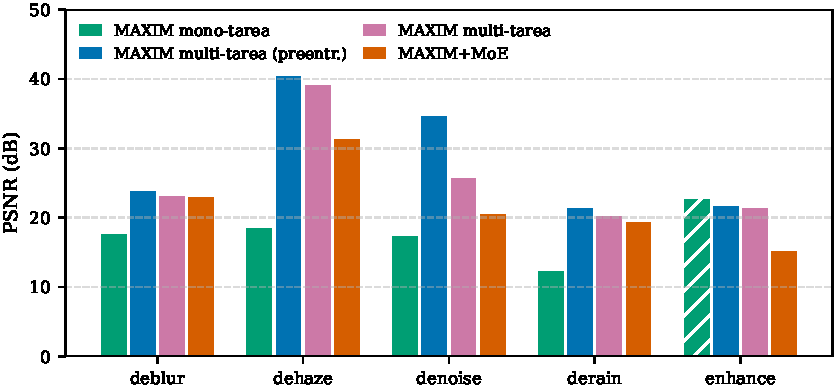
\includegraphics[width=0.85\textwidth]{figs/fig_task_comparison.pdf}
\caption{\label{fig:taskbars}PSNR por tarea de las cuatro configuraciones, según la evaluación a posteriori con protocolo homogéneo (mejor \textit{checkpoint} de cada modelo, submuestra aleatoria uniforme de hasta $200$ imágenes por tarea, recorte central de $256\times 256$). Al compartir protocolo, las cuatro barras de cada tarea son directamente comparables entre sí ---incluido el modelo mono-tarea, cuya tarea de entrenamiento (\textit{enhance}) se indica con rayado---, aunque, por el cambio de protocolo, las magnitudes no coinciden con la PSNR de validación del entrenamiento reportada en la Tabla~\ref{tab:cuant}. El modelo mono-tarea solo es competitivo en su tarea; la variante MoE acompaña al \textit{baseline} multi-tarea en \textit{deblurring} y \textit{deraining}, pero queda por debajo en \textit{dehazing}, \textit{denoising} y, sobre todo, realce.}
\end{figure*}

\begin{table*}[ht]
\caption{\label{tab:cuant}Comparación cuantitativa sobre el conjunto de validación (parches de $256\times 256$). Se reporta la mejor PSNR alcanzada, la SSIM asociada y la pérdida L1 de validación. ``Escala'' indica la variante de MAXIM (S-2 o S-3, según el número de etapas); ``Inic.'' la inicialización (aleatoria o desde \textit{checkpoint} preentrenado) y ``Sup.'' el tipo de supervisión (multi-escala o de una sola escala). La PSNR y la L1 corresponden a la validación durante el entrenamiento (conjunto mezclado, muestreo proporcional); la SSIM se calcula a posteriori con el mejor \textit{checkpoint} de cada configuración, promediando por tarea sobre una submuestra aleatoria uniforme de hasta $200$ imágenes por tarea (recorte central de $256\times 256$).}
\begin{ruledtabular}
\begin{tabular}{lcccccc}
Modelo & Escala & Inic. & Sup. & PSNR (dB) & SSIM & L1 val. \\
\hline
MAXIM mono-tarea\footnotemark[1]   & S-2 & aleat.   & multi  & $24{,}0$ & $0{,}871$ & $0{,}059$ \\
MAXIM multi-tarea  & S-3 & preentr. & multi  & $\mathbf{25{,}5}$ & $\mathbf{0{,}823}$ & $\mathbf{0{,}042}$ \\
MAXIM multi-tarea  & S-2 & aleat.   & multi  & $24{,}8$ & $0{,}754$ & $0{,}046$ \\
MAXIM+MoE          & S-2 & aleat.   & simple & $23{,}4$ & $0{,}678$ & $0{,}049$ \\
\end{tabular}
\end{ruledtabular}
\footnotetext[1]{El modelo mono-tarea se valida únicamente sobre su tarea de entrenamiento (\textit{enhance}); su PSNR y SSIM (medidas sobre esa tarea) no son directamente comparables con las filas multi-tarea, promediadas sobre las cinco tareas.}
\end{table*}

\begin{figure}[t]
\centering
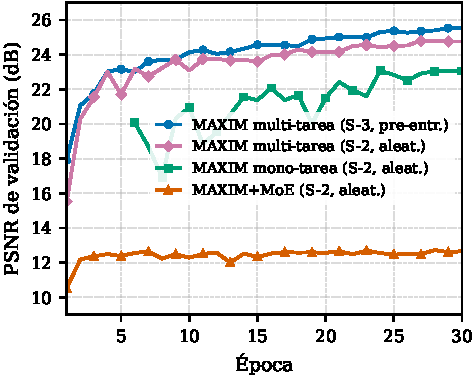
\includegraphics[width=\columnwidth]{figs/fig_val_psnr.pdf}
\caption{\label{fig:valpsnr}Evolución de la PSNR de validación durante el entrenamiento, para un presupuesto común de $30$ épocas. Las dos versiones multi-tarea de MAXIM sin MoE convergen a $24{,}8$--$25{,}5$~dB, y la mono-tarea alcanza $24{,}0$~dB sobre su única tarea (realce). La variante MAXIM+MoE converge a $23{,}4$~dB, aproximadamente $1{,}4$~dB por debajo de la multi-tarea desde cero, con la que comparte escala (S-2), inicialización aleatoria y datos, y que constituye por ello la comparación más justa.}
\end{figure}

\subsection{Dinámica de entrenamiento y comportamiento del ruteador}

La Fig.~\ref{fig:moedyn} examina con mayor detalle la corrida de MAXIM+MoE. El panel~(a) confirma que tanto la PSNR de entrenamiento como la de validación ascienden de forma conjunta y sostenida hasta estabilizarse cerca de $23$~dB; las curvas permanecen muy próximas entre sí, sin señales de sobreajuste. La pequeña oscilación periódica refleja la rotación entre las cinco tareas a lo largo de cada época. El backbone, por lo tanto, converge sin dificultad pese a la supervisión de una sola escala.

El panel~(b) revela el hallazgo central sobre el ruteador. La entropía de la distribución de compuerta asciende casi de inmediato hasta las inmediaciones de su valor máximo, $\ln K \approx 1{,}609$~nats, y allí se mantiene; en paralelo, el término de balance de carga permanece junto a su mínimo, $1{,}0$. En conjunto, ambos indicadores describen un ruteador que reparte su peso de forma prácticamente uniforme entre los cinco expertos (un uso medio de $0{,}2$ por experto, constante a lo largo de todo el entrenamiento). Es decir, el ruteador no llega a discriminar entre tareas ni tipos de degradación: la ``mezcla de expertos'' degenera en un promedio uniforme de cinco cabezas casi idénticas, equivalente en la práctica a una única cabeza de salida lineal sobre las características compartidas. La propuesta funciona, entonces, pero no como una verdadera mezcla de expertos.

\begin{figure*}[t]
\centering
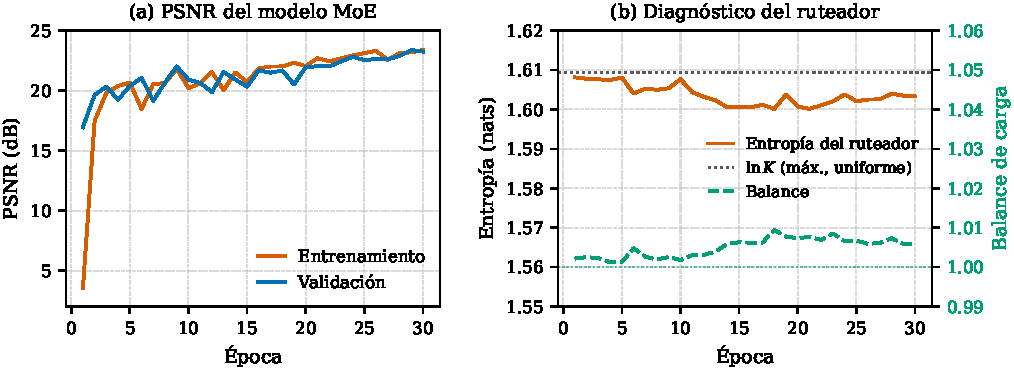
\includegraphics[width=\textwidth]{figs/fig_moe_dynamics.pdf}
\caption{\label{fig:moedyn}Diagnóstico de la variante MAXIM+MoE a lo largo de las $30$ épocas de entrenamiento. (a)~La PSNR de entrenamiento y validación convergen de forma conjunta hasta $\sim\!23$~dB, sin señales de sobreajuste. (b)~Ejes ampliados: la entropía del ruteador (naranja) permanece durante toda la corrida junto a su máximo $\ln K$ (línea punteada gris) y el balance de carga (verde) junto a su mínimo $1{,}0$: el ruteo se mantiene prácticamente uniforme y no emerge especialización entre expertos.}
\end{figure*}

Este patrón es coherente con la regularización empleada: tanto el premio a la entropía como la penalización del desbalance tienen su óptimo en la distribución uniforme, de modo que ambos términos empujan al ruteador hacia el mismo punto. Al no existir una señal que incentive la especialización ---por ejemplo, una supervisión explícita de la tarea sobre el ruteador--- y al ser el ruteo denso, la solución de mínimo esfuerzo consiste en igualar los pesos. El análisis de especialización por tipo de degradación, previsto inicialmente, pierde sentido en este escenario: sin asignaciones diferenciadas no emergen expertos asociados a degradaciones específicas.

\subsection{Resultados cualitativos}

La Fig.~\ref{fig:cualit} contrasta reconstrucciones sobre muestras representativas de validación, ordenadas en columnas: la entrada degradada, la salida del modelo base multi-tarea desde cero (S-2, la comparación justa), la de la variante MAXIM+MoE y la imagen de referencia. La comparación visual es consistente con la evaluación por tarea: en las degradaciones donde ambos modelos son cuantitativamente parejos ---\textit{deblurring}, \textit{deraining}--- las reconstrucciones son muy similares, mientras que en las tareas donde el MoE queda por debajo ---realce, \textit{denoising}--- su salida se ve más apagada y con menor detalle fino que la del modelo base. Este comportamiento es el esperable de un ruteador que promedia de manera uniforme cinco cabezas equivalentes, en lugar de seleccionar una hipótesis de reconstrucción especializada para cada entrada.

% NOTA: el figure* (doble columna) se declara ANTES que el figure de una
% columna a propósito. Los flotantes a doble columna sólo pueden ir en la
% banda superior de una página; si el figure de una columna reclama antes
% la cabecera de la columna izquierda, el figure* queda diferido a la
% página siguiente (que es lo que ocurría: Fig. de realce sola al final).
\begin{figure*}[t]
\centering
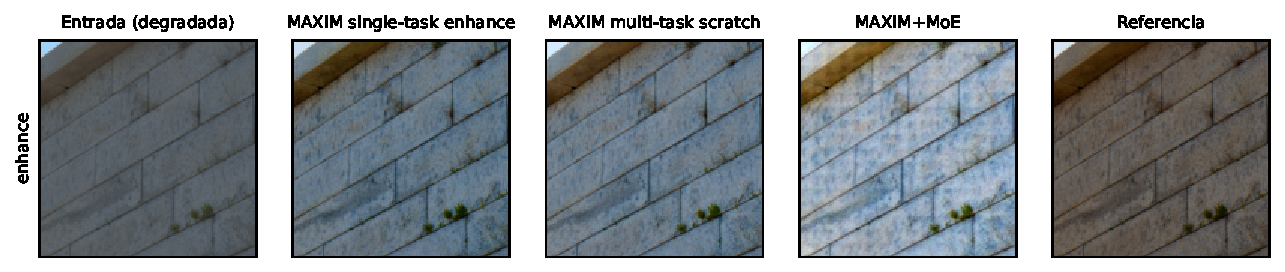
\includegraphics[width=0.85\textwidth]{figs/fig_qualitative_enhance.pdf}
\caption{\label{fig:cualit_enh}Comparación cualitativa sobre la tarea \textit{enhance}, la única en la que el modelo mono-tarea es directamente comparable. De izquierda a derecha: entrada degradada, MAXIM mono-tarea, MAXIM multi-tarea, MAXIM+MoE e imagen de referencia.}
\end{figure*}

\begin{figure}[t]
\centering
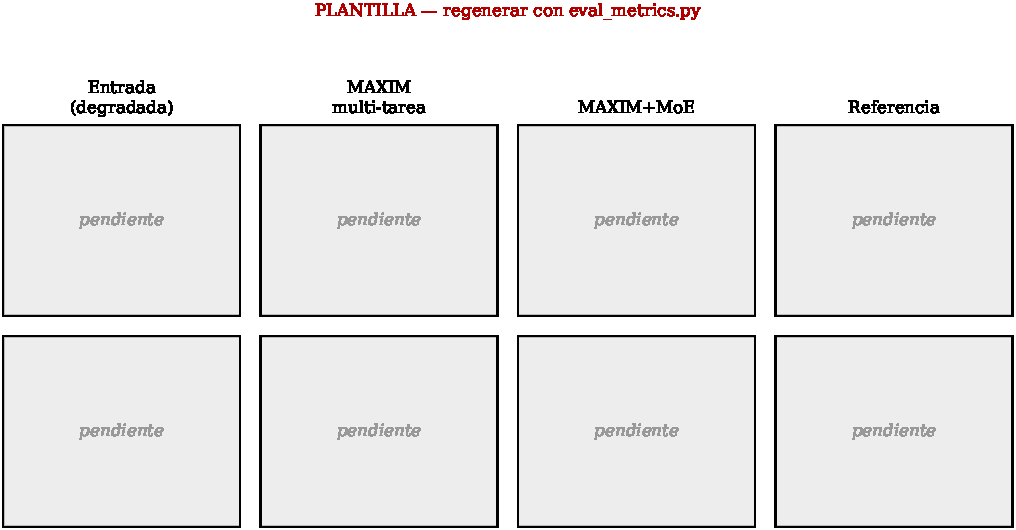
\includegraphics[width=\columnwidth]{figs/fig_qualitative.pdf}
\caption{\label{fig:cualit}Comparación cualitativa sobre muestras de validación de distintas tareas. De izquierda a derecha: entrada degradada, MAXIM multi-tarea desde cero (S-2), MAXIM+MoE e imagen de referencia.}
\end{figure}

El modelo mono-tarea se omite de la Fig.~\ref{fig:cualit} porque, al estar especializado únicamente en la tarea \textit{enhance}, su reconstrucción carece de sentido sobre las demás degradaciones. Para una comparación justa, la Fig.~\ref{fig:cualit_enh} restringe el contraste a esa tarea e incorpora su salida junto a las del modelo multi-tarea y la variante MAXIM+MoE. Sobre la tarea de realce, tanto el especialista mono-tarea como el modelo multi-tarea producen reconstrucciones fieles ($21{,}5$--$22{,}8$~dB), mientras que la variante MoE queda claramente por detrás ($15{,}3$~dB): es precisamente en esta tarea ---la que más se beneficiaría de una cabeza especializada--- donde la ausencia de especialización del ruteador resulta más costosa.

\section{Discusión}

Los resultados indican que, en la configuración evaluada, la variante MAXIM+MoE entrena de forma estable y produce reconstrucciones competentes, pero no mejora a la versión sin MoE: queda por debajo de todas las referencias. La comparación clave es con la versión multi-tarea entrenada desde cero, diseñada precisamente para eliminar factores de confusión: comparte con la variante MoE la escala del backbone (S-2), la inicialización aleatoria, el conjunto de entrenamiento y validación y el presupuesto de $30$ épocas. Su única diferencia es el esquema de expertos con supervisión de una sola escala. Como esa versión alcanza $24{,}8$~dB frente a los $23{,}4$~dB del MoE, la brecha ---aunque moderada--- no puede atribuirse ni al preentrenamiento ni al tamaño del modelo: proviene del propio esquema de expertos.

El punto central no es la magnitud de la brecha sino su origen. El análisis del ruteador (Fig.~\ref{fig:moedyn}) muestra que la mezcla nunca se activa como tal: el ruteo converge a un régimen prácticamente uniforme, de modo que las cinco cabezas se promedian y el modelo se comporta como si tuviera una única cabeza de salida lineal. La especialización que motivaba la propuesta no llega a emerger. Identificamos dos factores, propios de la variante MoE, que explican por qué:

\begin{enumerate}
    \item \textbf{Regularización que premia la uniformidad.} El término de entropía (maximizado) y el de balance de carga (que es mínimo en la distribución uniforme) tienen su óptimo en el mismo punto. En ausencia de una señal que favorezca la concentración del ruteo, ambos términos arrastran al ruteador hacia pesos iguales, que es exactamente el régimen no especializado que se buscaba evitar.
    \item \textbf{Ruteo denso sobre expertos de capacidad mínima.} Cada experto es una sola convolución $3\times 3$ y todos se evalúan y promedian en cada paso (ruteo denso). Partiendo de inicializaciones similares, cabezas tan simples reciben gradientes casi idénticos y no tienen incentivo ni margen para diferenciarse; permanecen intercambiables. Aun si el ruteo discriminara, una proyección lineal de las características compartidas difícilmente representaría reconstrucciones específicas por tarea.
\end{enumerate}

La consecuencia se observa en la evaluación por tarea: el MoE iguala al \textit{baseline} donde una única hipótesis de reconstrucción alcanza (\textit{deblurring}, \textit{deraining}) y solo se queda atrás donde haría falta una respuesta especializada (realce, \textit{denoising}, \textit{dehazing}). La pérdida de la supervisión profunda multi-escala de MAXIM ---la variante toma solo las características finales del backbone y usa una pérdida de una sola escala--- probablemente contribuye también a esa brecha residual, aunque, a diferencia de lo que anticipábamos, no impide que el backbone converja. Descartamos, por su parte, que el problema provenga de las condiciones compartidas de entrenamiento (inicialización aleatoria y \textit{batch} de tamaño $2$), ya que la versión multi-tarea desde cero opera bajo esas mismas condiciones y converge por encima. El sobrecosto de la propuesta sobre el backbone es marginal ---los expertos añaden una cantidad de parámetros despreciable---, de modo que el problema no es de eficiencia sino de eficacia: la especialización, no la convergencia, es lo que no llegó a materializarse.

Como subproducto, el trabajo deja líneas base sólidas y reproducibles: versiones multi-tarea de MAXIM que alcanzan entre $24{,}8$ y $25{,}5$~dB sobre la mezcla de cinco tareas ---con y sin preentrenamiento--- y una versión mono-tarea de referencia. Todas resultan útiles como punto de comparación para futuras variantes.

\section{Conclusiones}

El objetivo general de este trabajo fue evaluar si dotar a MAXIM de un esquema de Mixture of Experts en la etapa de reconstrucción aporta frente a una versión sin MoE. La evidencia experimental responde de forma negativa para la configuración estudiada: si bien la variante MAXIM+MoE entrena de forma estable y alcanza $23{,}4$~dB de PSNR de validación ---un restaurador competente, en el rango de las versiones multi-tarea sin MoE ($24{,}8$--$25{,}5$~dB)---, no las supera; en particular, una versión sin MoE de idéntica escala e inicialización alcanza $24{,}8$~dB, lo que aísla el origen de la brecha en el diseño de la propuesta y no en factores de confusión.

El hallazgo principal no es, sin embargo, la diferencia de PSNR, sino que la mezcla de expertos nunca se activa como tal. El ruteador converge a un régimen prácticamente uniforme ---entropía junto a su máximo $\ln K$ y balance de carga junto a su mínimo---, de modo que las cinco cabezas se promedian y equivalen a una única salida lineal; la especialización buscada nunca emerge. Este comportamiento es atribuible a una regularización cuyo óptimo es la distribución uniforme y a un ruteo denso sobre expertos lineales de capacidad mínima, que carecen de incentivo y de margen para diferenciarse. Consistentemente, el déficit frente al \textit{baseline} se concentra en las tareas que más se beneficiarían de una respuesta especializada (realce, \textit{denoising}), y es casi nulo donde una única hipótesis de reconstrucción alcanza.

El alcance del modelo implementado es, por lo tanto, limitado: tal como está formulado, el esquema de expertos de salida no aprovecha el potencial de la idea de especialización, aunque tampoco la degrada respecto de un modelo de una sola cabeza. El trabajo cumple así un propósito de delimitación: identifica con precisión qué condiciones impiden que la especialización emerja y, con ello, qué habría que cambiar para que la especialización tardía por expertos sea viable en restauración de imágenes. Las líneas base entrenadas como referencia constituyen, además, un aporte concreto y reutilizable.

\section{Trabajo futuro}

El análisis sugiere intervenciones directas para una próxima iteración; las dos primeras atacan la causa central ---que el ruteo no se especializa--- y son, por lo tanto, prioritarias:
\begin{itemize}
    \item \textbf{Replantear la regularización del ruteo.} Reducir o eliminar el premio a la entropía, calibrar el balance de carga para evitar que domine la pérdida, y considerar una supervisión explícita de la tarea sobre el ruteador o un ruteo disperso (top-1/top-2) que fuerce decisiones discriminativas~\cite{shazeer2017moe,fedus2022switch}. Es la palanca más directa contra el régimen uniforme.
    \item \textbf{Aumentar la capacidad de los expertos y romper su simetría.} Reemplazar la convolución única por cabezas con varias capas o bloques residuales, de modo que cada experto pueda representar reconstrucciones realmente distintas, e inicializarlas de forma diferenciada para que no reciban gradientes idénticos; explorar además la incorporación de expertos en etapas internas del backbone.
    \item \textbf{Preservar la supervisión profunda.} Conservar las salidas multi-etapa y multi-escala de MAXIM, o aplicar la mezcla de expertos sobre cada escala supervisada, para cerrar la brecha residual frente al \textit{baseline} multi-escala.
    \item \textbf{Inicializar desde pesos preentrenados.} Partir del \textit{backbone} preentrenado de MAXIM, como en la línea base multi-tarea, y reservar el entrenamiento desde cero solo para el ruteador y los expertos.
    \item \textbf{Mejorar las condiciones de optimización y la evaluación.} Emplear acumulación de gradiente o \textit{hardware} con más memoria para entrenar con \textit{batches} efectivos mayores, y complementar PSNR y SSIM con métricas perceptuales basadas en redes (LPIPS) y evaluación a resolución completa.
\end{itemize}

%\section{Aknowledgments}
\section{Agradecimientos}

\begin{acknowledgments}
\end{acknowledgments}
% Referencias.
% Se incluyen en línea (entorno thebibliography) para que el documento compile
% con pdflatex sin depender del paso de BibTeX. Si se prefiere usar BibTeX,
% comentar el bloque thebibliography y descomentar la línea siguiente
% (el archivo ref.bib está disponible en este directorio):
% \bibliography{ref}

\begin{thebibliography}{99}

\bibitem{tu2022maxim}
Z.~Tu, H.~Talebi, H.~Zhang, F.~Yang, P.~Milanfar, A.~Bovik, and Y.~Li,
\textit{MAXIM: Multi-Axis MLP for Image Processing},
in Proc. IEEE/CVF Conf. on Computer Vision and Pattern Recognition (CVPR) (2022), pp. 5769--5780.

\bibitem{jacobs1991mixtures}
R.~A. Jacobs, M.~I. Jordan, S.~J. Nowlan, and G.~E. Hinton,
\textit{Adaptive Mixtures of Local Experts},
Neural Comput. \textbf{3}, 79 (1991).

\bibitem{shazeer2017moe}
N.~Shazeer, A.~Mirhoseini, K.~Maziarz, A.~Davis, Q.~Le, G.~Hinton, and J.~Dean,
\textit{Outrageously Large Neural Networks: The Sparsely-Gated Mixture-of-Experts Layer},
in Proc. Int. Conf. on Learning Representations (ICLR) (2017).

\bibitem{fedus2022switch}
W.~Fedus, B.~Zoph, and N.~Shazeer,
\textit{Switch Transformers: Scaling to Trillion Parameter Models with Simple and Efficient Sparsity},
J. Mach. Learn. Res. \textbf{23}, 1 (2022).

\bibitem{nah2017gopro}
S.~Nah, T.~H. Kim, and K.~M. Lee,
\textit{Deep Multi-scale Convolutional Neural Network for Dynamic Scene Deblurring},
in Proc. IEEE Conf. on Computer Vision and Pattern Recognition (CVPR) (2017).

\bibitem{wei2018lol}
C.~Wei, W.~Wang, W.~Yang, and J.~Liu,
\textit{Deep Retinex Decomposition for Low-Light Enhancement},
in Proc. British Machine Vision Conference (BMVC) (2018).

\bibitem{abdelhamed2018sidd}
A.~Abdelhamed, S.~Lin, and M.~S. Brown,
\textit{A High-Quality Denoising Dataset for Smartphone Cameras},
in Proc. IEEE Conf. on Computer Vision and Pattern Recognition (CVPR) (2018).

\bibitem{li2019reside}
B.~Li, W.~Ren, D.~Fu, D.~Tao, D.~Feng, W.~Zeng, and Z.~Wang,
\textit{Benchmarking Single-Image Dehazing and Beyond},
IEEE Trans. Image Process. \textbf{28}, 492 (2019).

\bibitem{fu2017derain}
X.~Fu, J.~Huang, D.~Zeng, Y.~Huang, X.~Ding, and J.~Paisley,
\textit{Removing Rain from Single Images via a Deep Detail Network},
in Proc. IEEE Conf. on Computer Vision and Pattern Recognition (CVPR) (2017).

\bibitem{loshchilov2019adamw}
I.~Loshchilov and F.~Hutter,
\textit{Decoupled Weight Decay Regularization},
in Proc. Int. Conf. on Learning Representations (ICLR) (2019).

\bibitem{wang2004ssim}
Z.~Wang, A.~C. Bovik, H.~R. Sheikh, and E.~P. Simoncelli,
\textit{Image Quality Assessment: From Error Visibility to Structural Similarity},
IEEE Trans. Image Process. \textbf{13}, 600 (2004).

\bibitem{zhang2018lpips}
R.~Zhang, P.~Isola, A.~A. Efros, E.~Shechtman, and O.~Wang,
\textit{The Unreasonable Effectiveness of Deep Features as a Perceptual Metric},
in Proc. IEEE/CVF Conf. on Computer Vision and Pattern Recognition (CVPR) (2018).

\bibitem{jax2018}
J.~Bradbury, R.~Frostig, P.~Hawkins, M.~J. Johnson, C.~Leary, D.~Maclaurin,
G.~Necula, A.~Paszke, J.~VanderPlas, S.~Wanderman-Milne, and Q.~Zhang,
\textit{JAX: Composable Transformations of Python+NumPy Programs} (2018),
\url{http://github.com/google/jax}.

\bibitem{flax2023}
J.~Heek, A.~Levskaya, A.~Oliver, M.~Ritter, B.~Rondepierre, A.~Steiner, and M.~van Zee,
\textit{Flax: A Neural Network Library and Ecosystem for JAX} (2023),
\url{http://github.com/google/flax}.

\end{thebibliography}

\end{document}
%
% ****** End of file apstemplate.tex ******
